% Created 2024-05-09 Thu 13:52
% Intended LaTeX compiler: pdflatex
\documentclass{beamer}
\usepackage[utf8]{inputenc}
\usepackage[T1]{fontenc}
\usepackage{graphicx}
\usepackage{longtable}
\usepackage{wrapfig}
\usepackage{rotating}
\usepackage[normalem]{ulem}
\usepackage{amsmath}
\usepackage{amssymb}
\usepackage{capt-of}
\usepackage{hyperref}
\usepackage{minted}
\usepackage{listings}
\usetheme{Boadilla}
\author{Kyle C. McGovern}
\date{}
\title{Scale Sensitivity as a Tool for Differential Set Analyses}
\institute[]{Silverman Lab \\ The Pennsylvania State University \\ Program in Bioinformatics and Genomics}

\AtBeginSection[]{\begin{frame}<beamer>\vfill\centering\usebeamerfont{title}\insertsectionhead\vfill\end{frame}}
\usepackage{pdfpages}
\setbeamercolor{background canvas}{bg=}
\makeatletter\beamer@ignorenonframefalse\makeatother
\usepackage{caption}
\usepackage{subcaption}
\usepackage{multicol}
\beamertemplatenavigationsymbolsempty
\usepackage{amssymb}
\definecolor{links}{HTML}{4167E1}
\hypersetup{colorlinks,linkcolor=,urlcolor=links}
\usepackage{lmodern}
\DeclareMathOperator*{\mean}{mean}
\DeclareMathOperator*{\median}{median}
\newcommand{\E}{\mathbb{E}} % Nice Infimum
\usefonttheme{professionalfonts}
%\setbeameroption{show notes on second screen=bottom} % Both
\usepackage[doi=false,isbn=false,url=false,eprint=false,style=authoryear]{biblatex}
\addbibresource{~/Dropbox/org/roam/references/references.bib}
\hypersetup{
 pdfauthor={Kyle C. McGovern},
 pdftitle={Scale Sensitivity as a Tool for Differential Set Analyses},
 pdfkeywords={},
 pdfsubject={},
 pdfcreator={Emacs 29.3 (Org mode 9.7-pre)}, 
 pdflang={English}}
\begin{document}

\maketitle
\note{
\begin{itemize}
\item Previously michelle introduced modifications of ALDEx2 (adding scale models) for DA/DE (LFC estimation)
\item Here we expand in two ways
\begin{enumerate}
\item we introduce sensitivity analyses as an alternative to the types of models michelle was discussing
\item we move to a different estimand DSA where goal is to determine if sets of genes/microbes are enriched (or depleted) between conditions.
\end{enumerate}
\end{itemize}}
\begin{frame}[label={sec:org0e992d4}]{Differential Set Analysis}
\vfill
\begin{block}{Differential (Expression/Abundance) Analysis}
Which Genes (or Taxa) are changing in amount between conditions? 
\end{block}
\vfill
\begin{block}{Differential Set Analysis}
\textcolor{gray}{aka Gene (or Microbe) Set Enrichment Analysis}

\medskip Which pathways (sets of genes) or sets of microbes are changing in amount between conditions?
\end{block}
\vfill
\note{
examples:
\begin{itemize}
\item glycogen degredation
\item anarobes
\end{itemize}}
\end{frame}
\section{Review and Problem Statement}
\label{sec:org2b19552}

\begin{frame}[label={sec:org82e28ba}]{Scale Reliant Inference}
\begin{align*}
  \underbrace{W_{dn}}_{\substack{\text{Absolute Abundance} \\ \text{Taxa d, Patient n}}} = \underbrace{W^\parallel_{dn}}_{\substack{\text{Composition} \\ \text{Taxa d, Patient n} }} \times \underbrace{W^\perp_n}_{\substack{\text{Scale} \\ \text{(e.g., total \# of microbes in} \\ \text{patient n's colon)}}}
\end{align*}

\pause
We measure sequence count data \(Y\) which provides information about \(W^{\parallel}\) but not \(W^{\perp}\).

\pause

\[\theta=f(W^{\parallel}, W^{\perp})\]
\pause
\begin{example}[Differential Abundance / Expression Analysis]\label{sec:orgd8e844c}
Using 16S rRNA-seq data, we want to identify which taxa change in abundance between cases and controls (LFC estimation).
\begin{align*}
  \theta_d = \mean_{n \in \text{case}}(\log W_{dn}) - \mean_{n \in \text{control}}(\log W_{dn} )
\end{align*}
\end{example}
\end{frame}
\begin{frame}[label={sec:org77ed647}]{Scale-Composition of LFC Estimand}
\begin{align*}
  \theta_d = \mean_{n \in \text{case}}(\log W_{dn}) - \mean_{n \in \text{control}}(\log W_{dn} )
\end{align*}


Using the relationship \(W_{dn} = W^\parallel_{dn} \times W^\perp_n\):
\small
\begin{align*}
  \small
  \theta_{d} &=  \underbrace{\left[\mean_{n \in \text{case}}(\log W^{\parallel}_{dn}) - \mean_{n \in \text{control}}(\log
  W^{\parallel}_{dn})\right]}_{\theta^\parallel_d}+\underbrace{\left[\mean_{n \in \text{case}}(\log W^{\perp}_{n}) - \mean_{n \in \text{control}}(\log W^{\perp}_{n})\right]}_{\theta^\perp} \label{eq:diff-analysis-2} \\
                       &= \theta_{d}^{\parallel}+\theta^\perp. \nonumber
\end{align*}

\pause

\begin{itemize}
\item \(\theta^{\parallel}_{d}\) is the LFC in composition of the \(d\)-th taxon \textcolor{gray}{(How do the proportions change between conditions?)}
\item \(\theta^{\perp}\) is the LFC in scales \textcolor{gray}{(How do the totals change between conditions?)}
\end{itemize}
\end{frame}
\begin{frame}[label={sec:orgc8a7a84}]{LFC Vector Notation}
\begin{align*}
  \begin{bmatrix} \theta_1 \\ \vdots \\ \theta_D \end{bmatrix} &= \begin{bmatrix} \theta^\parallel_1 \\ \vdots \\ \theta^\parallel_D \end{bmatrix} + \begin{bmatrix} 1 \\ \vdots \\ 1 \end{bmatrix} \theta^\perp \\
  \theta &= \theta^\parallel + \pmb{1}\theta^\perp
\end{align*}
\end{frame}
\section{LFC Sensitivity Analysis}
\label{sec:orgced24ba}
\begin{frame}[label={sec:org3f996c6}]{Scale Assumptions}
Methods like DESeq2 or ALDEx2 estimate LFCs (\(\hat{\theta}\)).
\[\hat{\theta}=\hat{\theta}^{\parallel} + \pmb{1}\hat{\theta}^{\perp}\]

\pause
\vfill
Because the data provides information about \(W^{\parallel}\), ignore error in \(\hat{\theta}^{\parallel}\)   (assuming \(\hat{\theta}^{\parallel}=\theta^{\parallel}\)).

\pause
\vfill
Since the data lacks information about \(\theta^{\perp}\) we call \(\hat{\theta}^{\perp}\) a \textit{\bf scale assumption}.

\pause
\vfill
Assumptions are subject to error \(\theta^{\perp}=\hat{\theta}^{\perp}+\epsilon^{\perp}\).

\pause
\vfill
\begin{block}{LFC Sensitivity Analysis}
\vspace{-2ex}
\begin{align*}
\theta &= \hat{\theta} + \mathbf{1}\epsilon^{\perp}
\end{align*}
\end{block}
\note{
When introducing scale assumptions mention that the assumption is often made by normalization (as michelle discussed). 

Final equation is key:
\begin{itemize}
\item ``This equation tells us how error in our assumptions about scale propagate into out LFC estimates.''
\end{itemize}}
\end{frame}
\begin{frame}[label={sec:orgd1abbf4}]{Review Scale Assumptions}
\vfill
\begin{itemize}
\item CLR Normalization (\(W^{\perp}_{n}=1/GM(W^{\parallel}\cdot n)\)) leads to
\end{itemize}
\[\hat{\theta}^{\perp}_{\text{CLR}} = \mean_{case}\log(1/GM(W^{\parallel}_{\cdot n}))-\mean_{control}\log (1/GM(W^{\parallel}_{\cdot n}))\]
\vfill
\begin{itemize}
\item TSS Normalization (dividing by sequencing depth) implies
\end{itemize}
\[\hat{\theta}^{\perp}_{\text{TSS}}=0\] 
\vfill
\end{frame}
\begin{frame}[label={sec:org130c059}]{LFC Sensitivity Analysis is Boring on Its Own}
\[\theta_{d}=\hat{\theta}_{d}+\epsilon^{\perp}\]
\vfill
\begin{center}
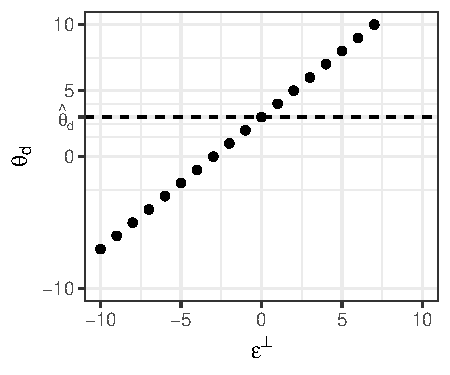
\includegraphics[width=0.6\linewidth]{da_lfc_sensitivity.pdf}
\label{org19f4bf0}
\end{center}
\end{frame}
\begin{frame}[label={sec:orgc1381d6}]{Aside: Interpretation of \(\epsilon^{\perp}\)}

At a given level of error \(\epsilon^\perp\), the true ratio of the average scale in case vs. control is \(e^{\epsilon^\perp}\) higher than assumed. 

\vfill
\begin{example}[]\label{sec:orgab734cb}
If \(\epsilon^\perp=1\) then the true average scale (ratio) is \(e^{1}\approx 2.7\) times higher than assumed. 
\end{example}
\end{frame}
\section{Differential Set Analysis (DSA)}
\label{sec:org1ac33bd}
\begin{frame}[label={sec:orgc1038f9}]{Target Estimand for DSA}
Let \(S\)  be a set of genes or microbes e.g., \(S=\{\text{Taxa 1}, \text{Taxa 3}, \text{Taxa 9}\}\)


\vspace{15px}

The goal of DSA is to infer \(\phi_S\) where
\begin{align*}
  \phi_S = \begin{cases}
    1 & \text{If } S \text{ is enriched} \\
    -1 & \text{If } S \text{ is depleted} \\
    0 & \text{If } S \text{ is neither enriched/depleted}
  \end{cases}
\end{align*}

\vspace{15px}
\pause
\begin{itemize}
\item Many researchers define \(\phi_{S}\) as a function of \(\theta\) (LFCs) which in turn is a function of \(W\):
\end{itemize}
\[\phi_{S}=u(\theta).\]

\begin{itemize}
\item Particularly common is defining \(u\) based on the GSEA algorithm.
\end{itemize}
\end{frame}
\begin{frame}[label={sec:org99a194f}]{Gene (and Microbe) Set Enrichment Analysis (GSEA)}
\begin{columns}
\begin{column}{0.5\columnwidth}
\begin{center}
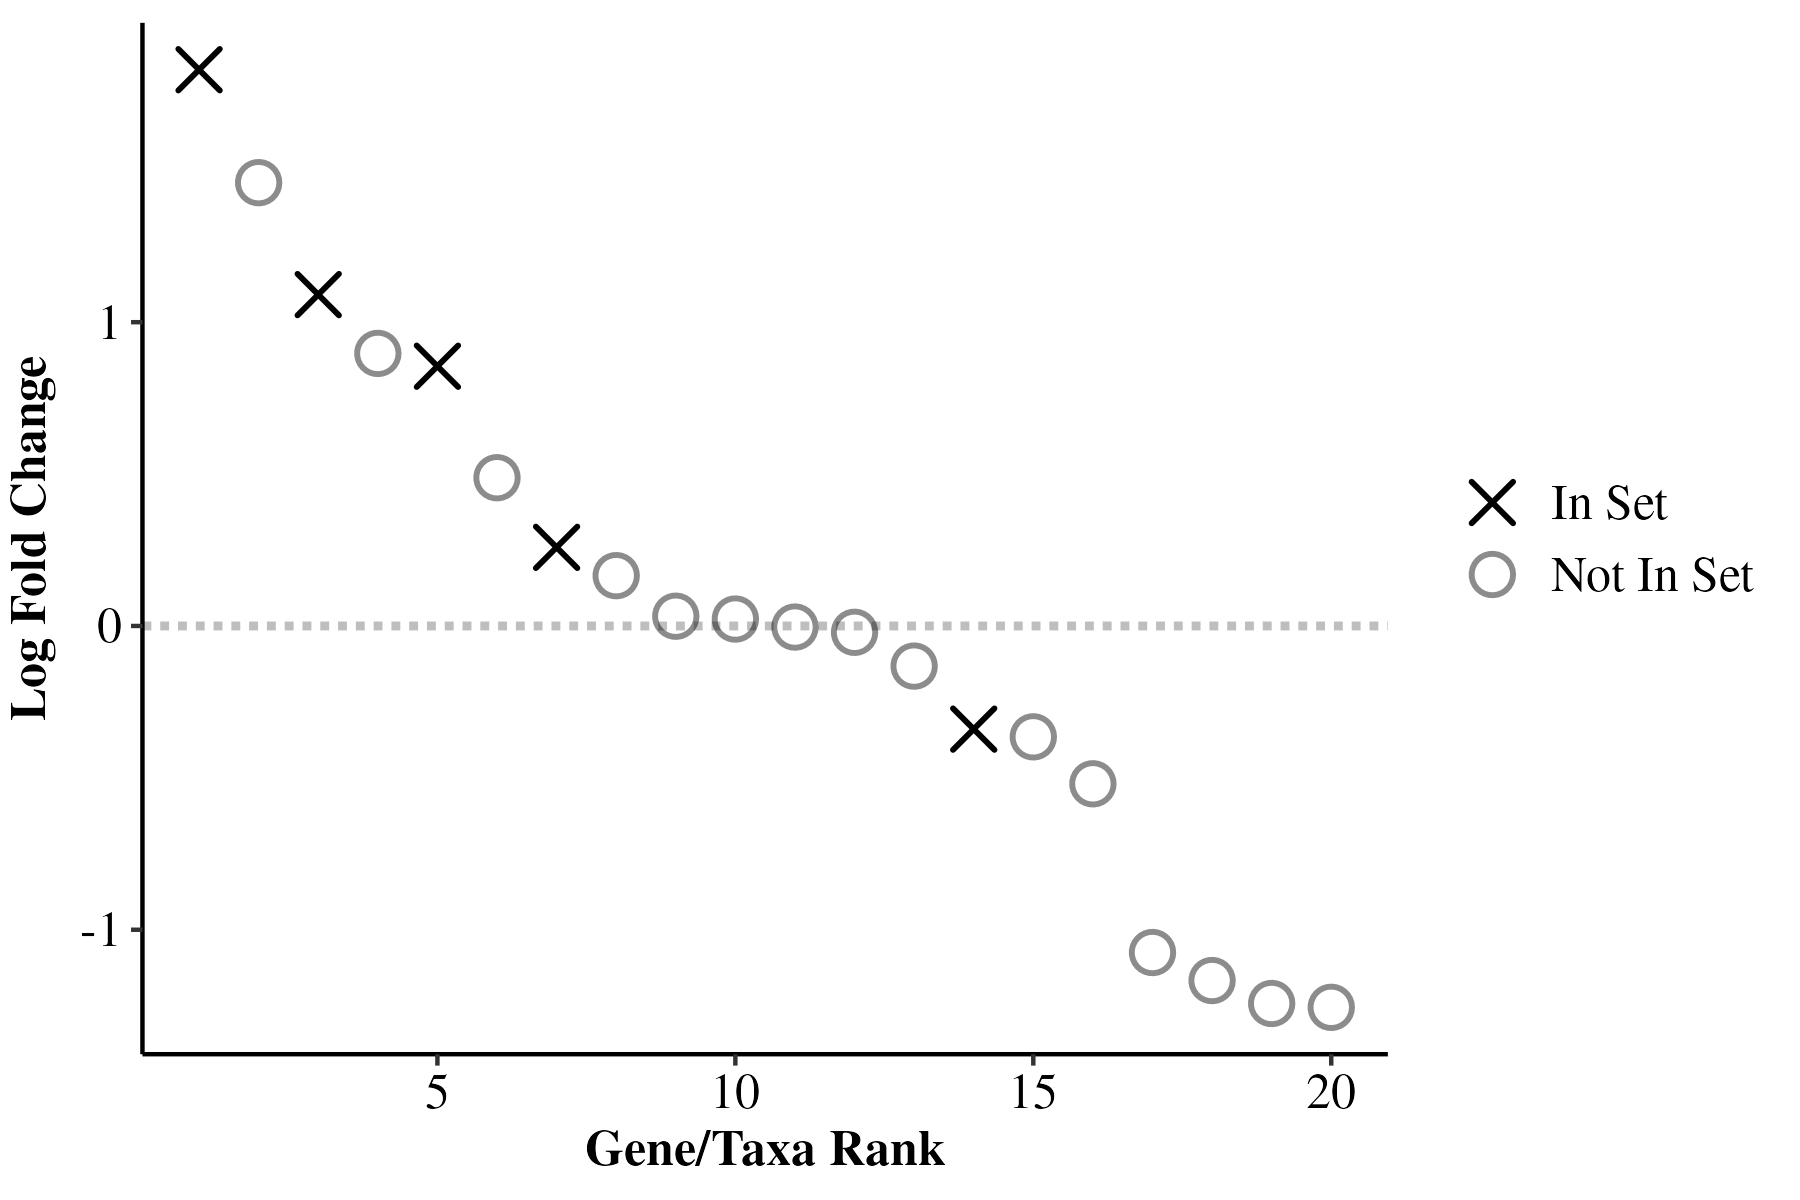
\includegraphics[width=0.85\linewidth]{./images/lfcs_1.png}
\end{center}
\pause
\begin{center}
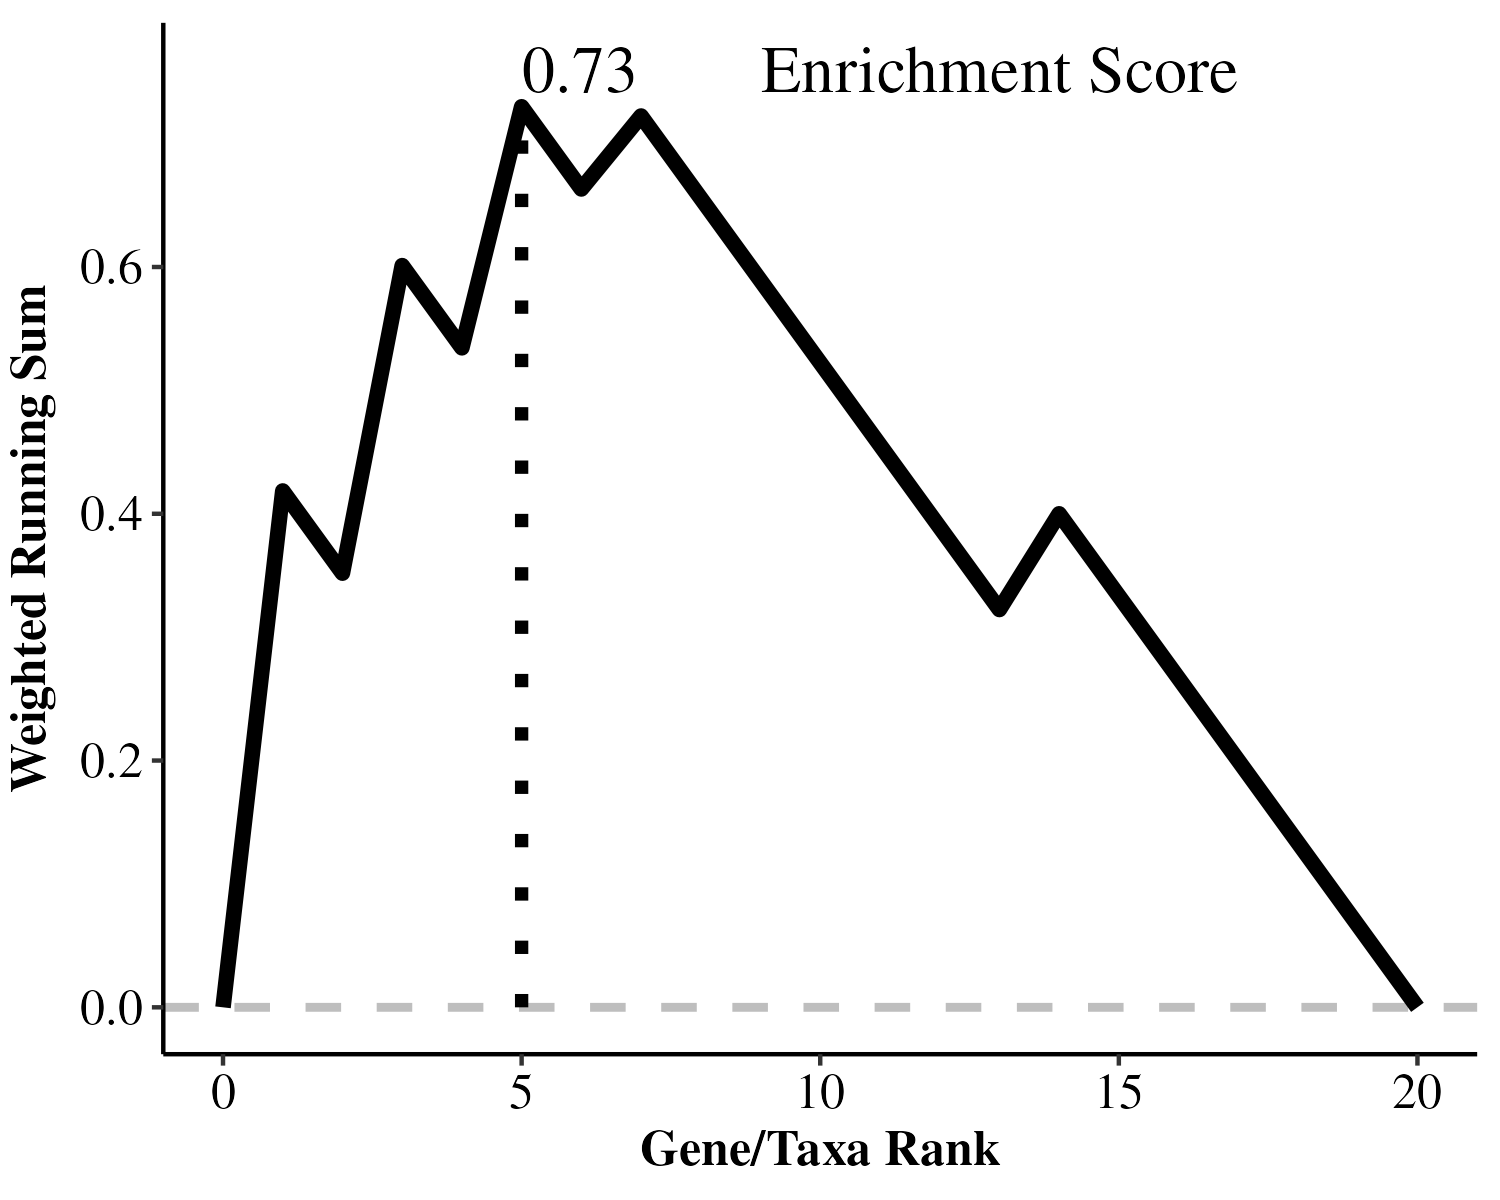
\includegraphics[width=0.85\linewidth]{./images/lfcs_2.png}
\end{center}
\end{column}
\begin{column}{0.5\columnwidth}
\pause
Statistical significance (p-values) estimated by permutation test:

\vfill

\textbf{Gene Label permutations}
\begin{itemize}
\item Our focus to start
\item Computationally simpler
\item Requires less data
\item Ignores for inter-gene (or inter-taxa) correlations
\end{itemize}

\vfill

\textbf{Sample Label permutations}
\begin{itemize}
\item Discussed later
\end{itemize}
\end{column}
\end{columns}
\note{
\begin{itemize}
\item After first figure, explain intuition -- we want a statistic that captures clustering at top or bottom of the list.

\item as you walk through pay special attention to explain how the running sum - if there was no clustering and X's are randomly distributed - would oscillate around zero and never deviate much.

\item don't forge to explain what gene/sample label permutations are
\end{itemize}}
\end{frame}
\begin{frame}[label={sec:org8d9f660}]{LFC Sensitivity Analysis for GSEA}
\[\phi_{S}=u(\theta)\]

\vfill
\pause
\begin{block}{}
\vspace{-1ex}
\[\phi_{S}=u(\hat{\theta}+\mathbf{1}\epsilon^{\perp})\]
\end{block}
\note{
Don't go to fast here, emphasize importance and explain:
We can study how conclusions about enrichment/depletion change with different levels of error.}
\end{frame}
\begin{frame}[label={sec:orgfcca331}]{Simulated Data Example}
\begin{center}
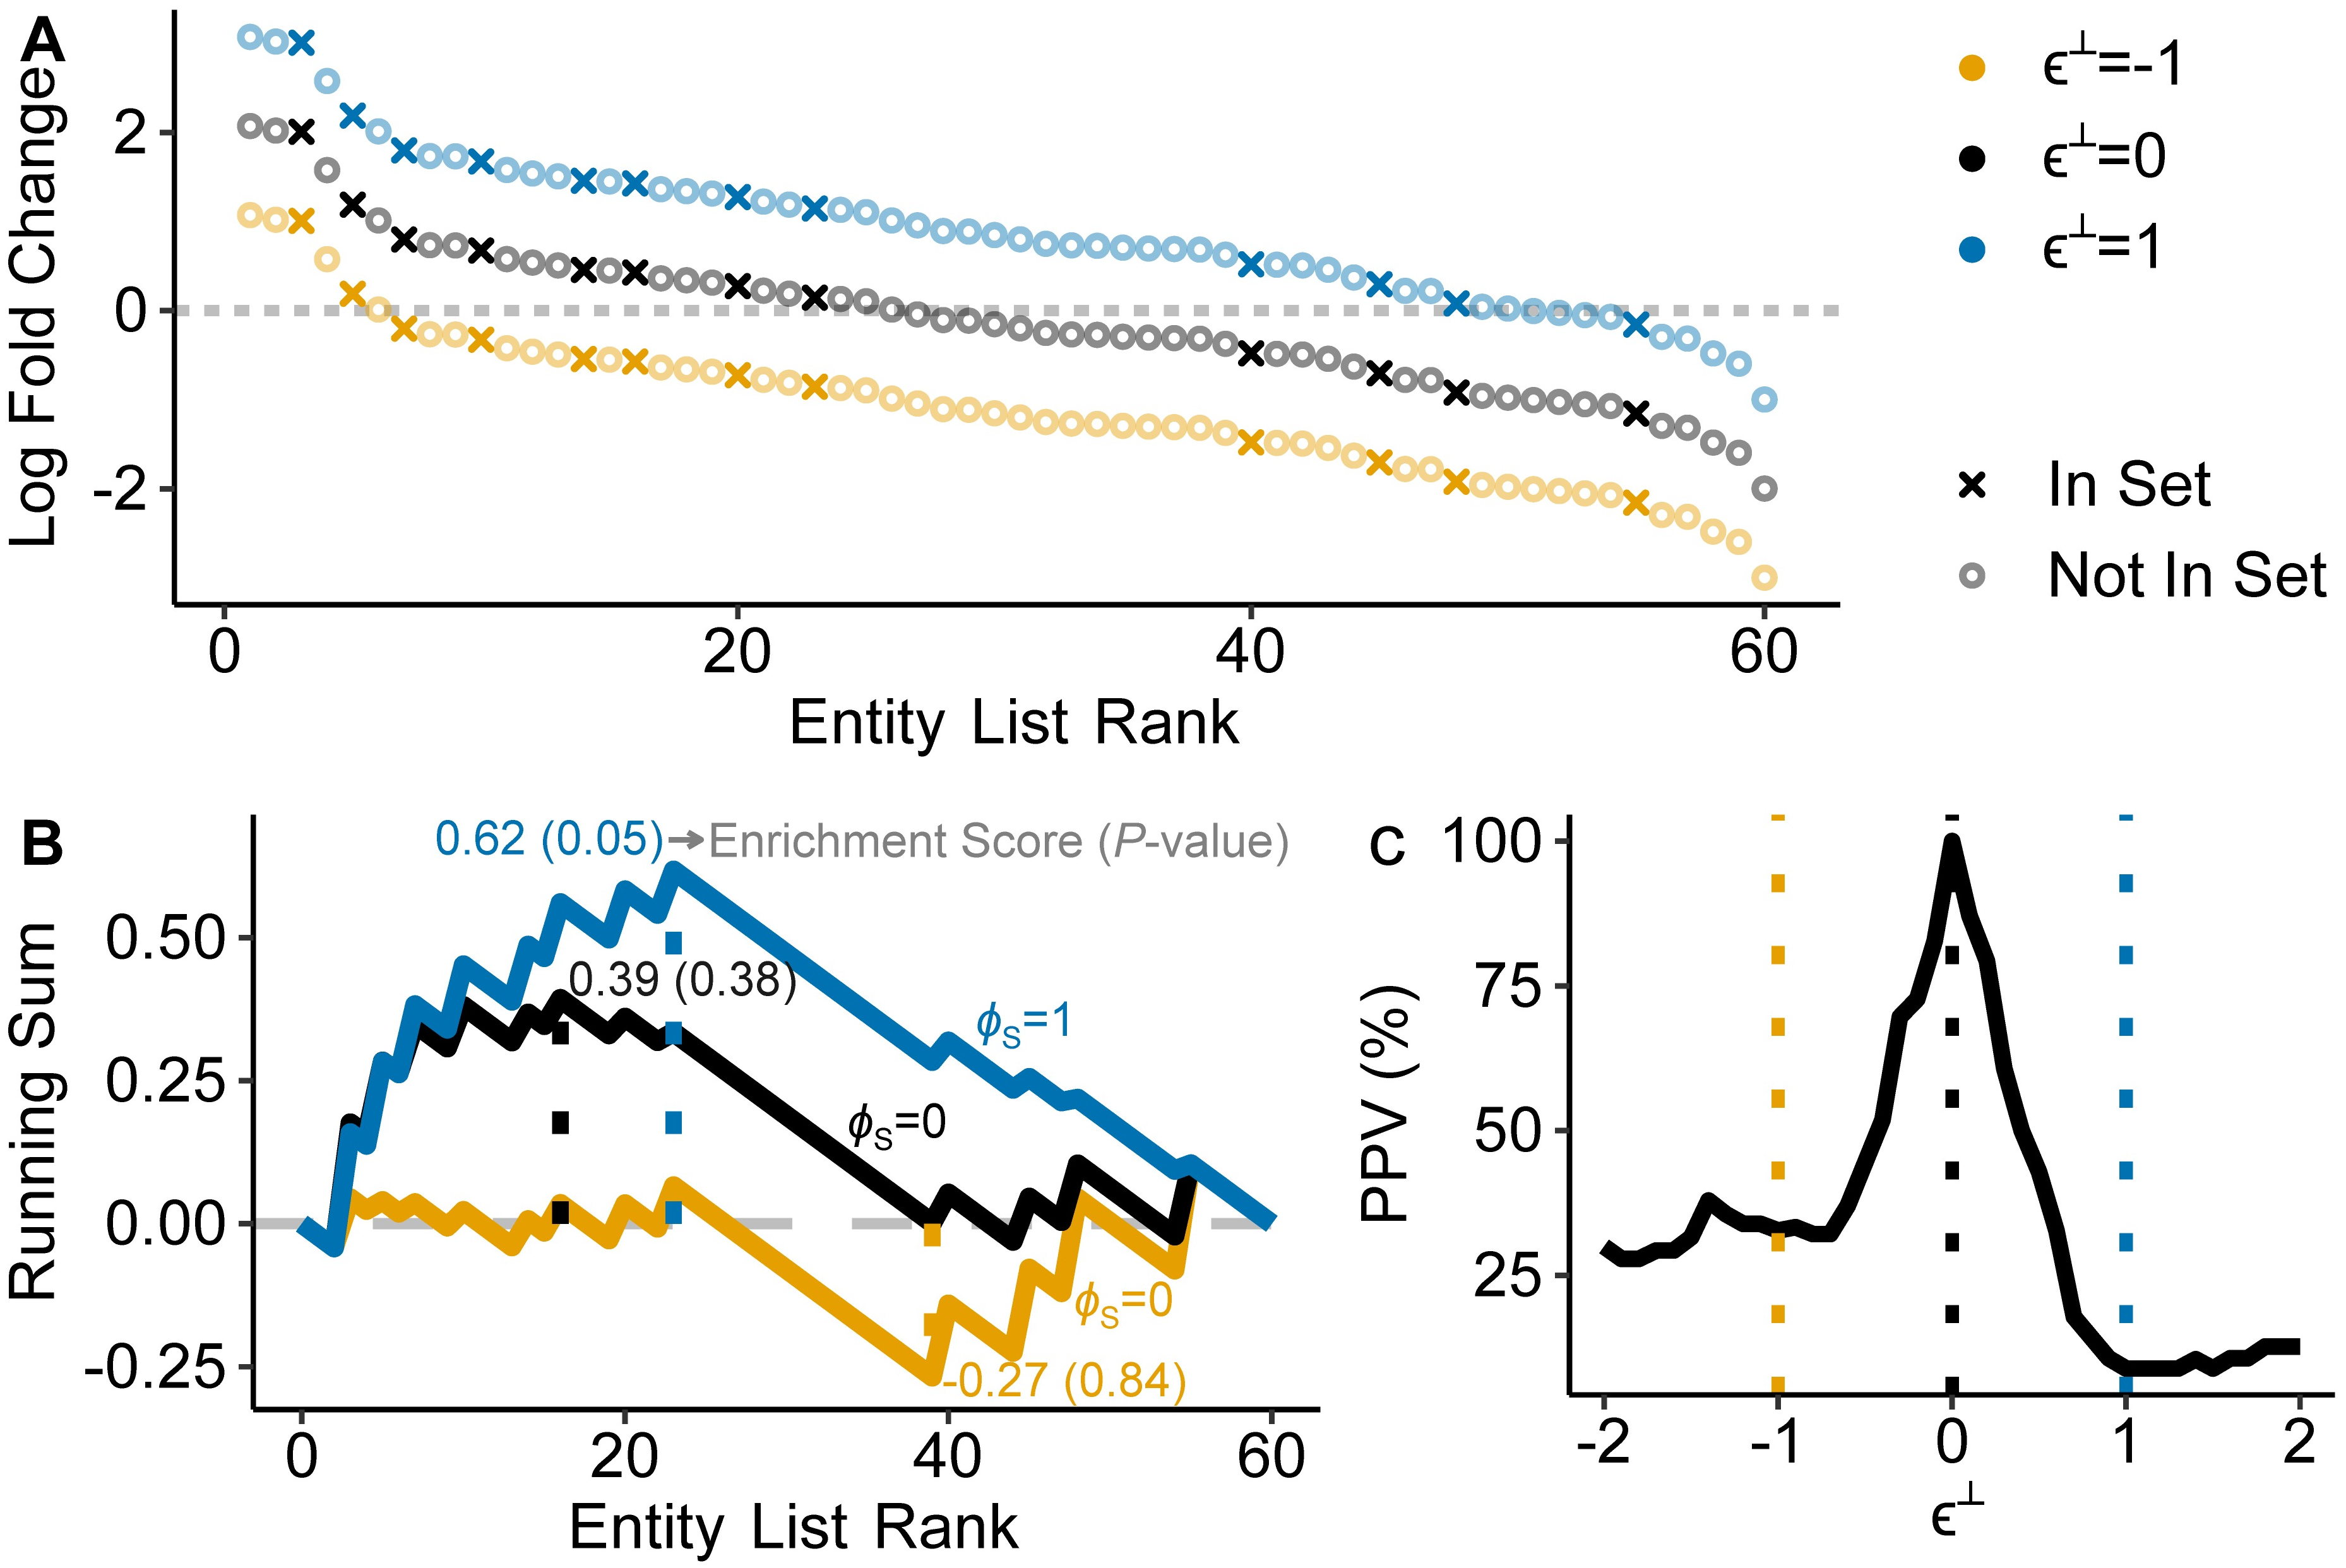
\includegraphics[width=0.9\linewidth]{./images/first_fig.png}
\end{center}
\note{
either hide PPV plot at start or explciitly tell people to ignore it at first, that you will explain it in a minute.}
\end{frame}
\begin{frame}[label={sec:org87568f7}]{Real Data Example}
\begin{columns}
  \begin{column}{0.5\textwidth}
   \begin{center}
     \underline{Healthy}
     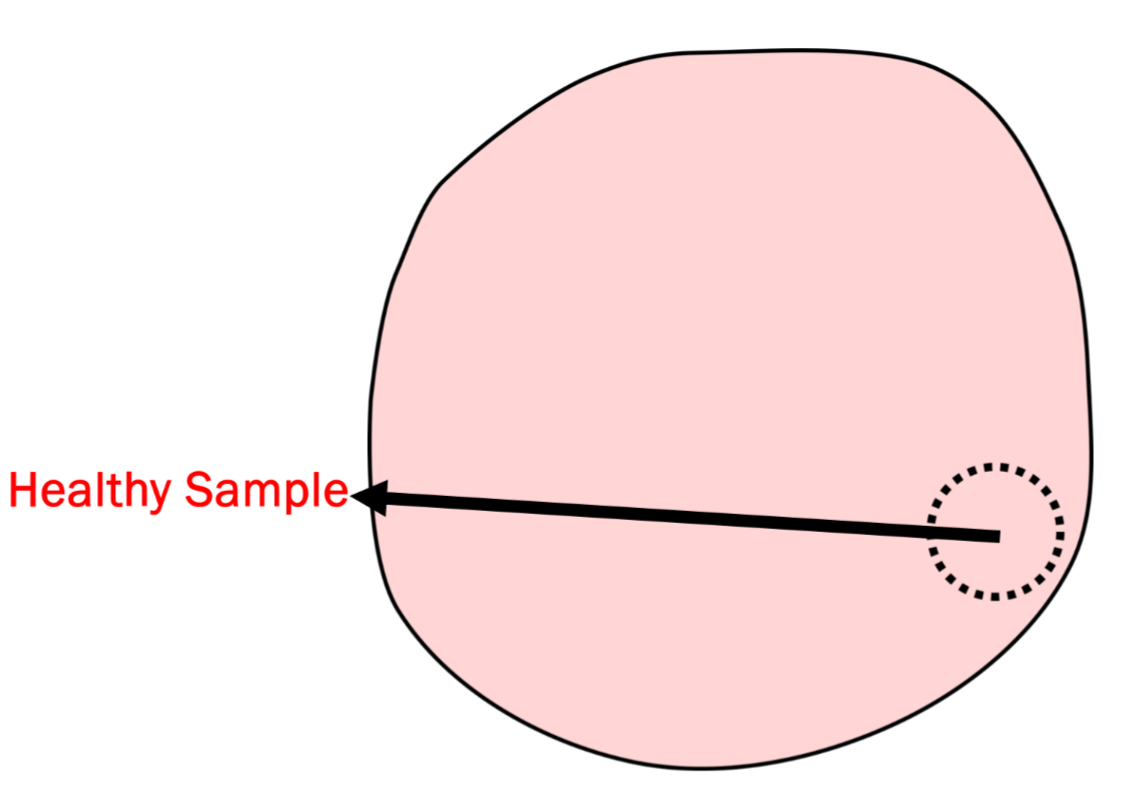
\includegraphics[scale=0.12]{./images/healthy.png}
   \end{center}
 \end{column}
 \vrule{}
 \begin{column}{0.5\textwidth}  %%<--- here
   \begin{center}
     \underline{Normal-Adjacent-to-Tumor (NAT)}
     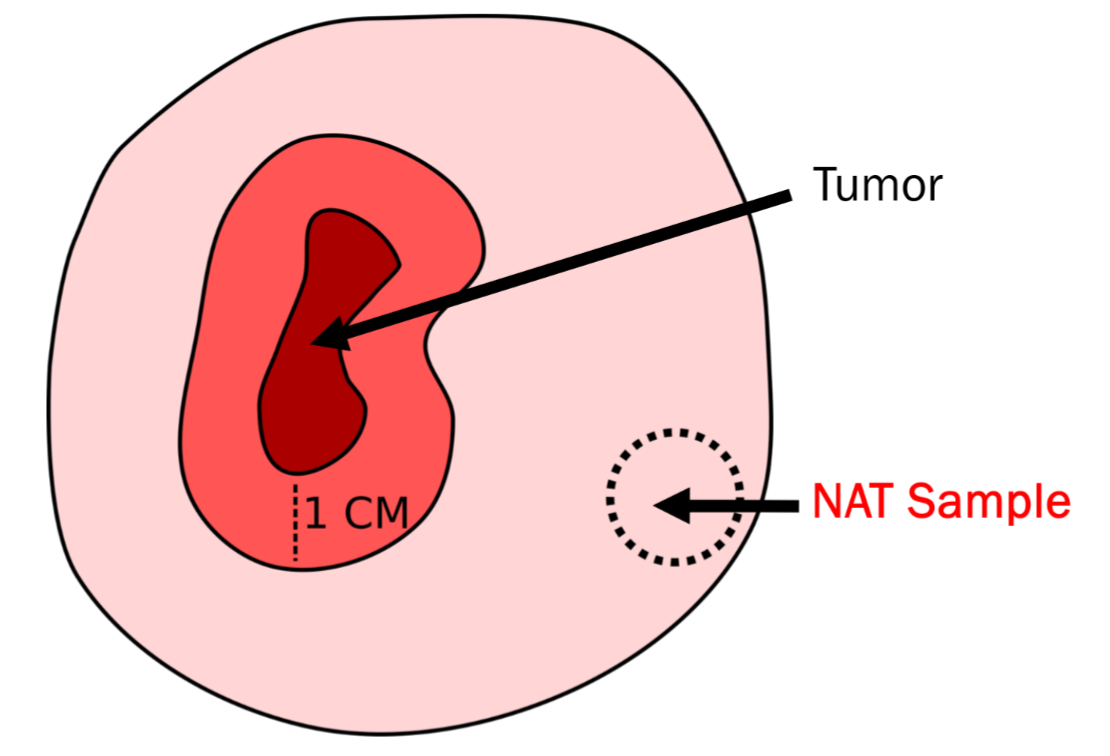
\includegraphics[scale=0.12]{./images/nat.png}
   \end{center}
 \end{column}
\end{columns}
\begin{block}{Motivation}
\begin{itemize}
\item Normal Adjacent to Tumor (NAT) is often used as surrogate for healthy control.
\item But is it really the same as healthy tissue?
\item We reanalyze RNA-seq data from healthy verus NAT thyroid tissue.
\end{itemize}
\end{block}
\end{frame}
\begin{frame}[label={sec:org975d291}]{Real Data Example}
\begin{center}
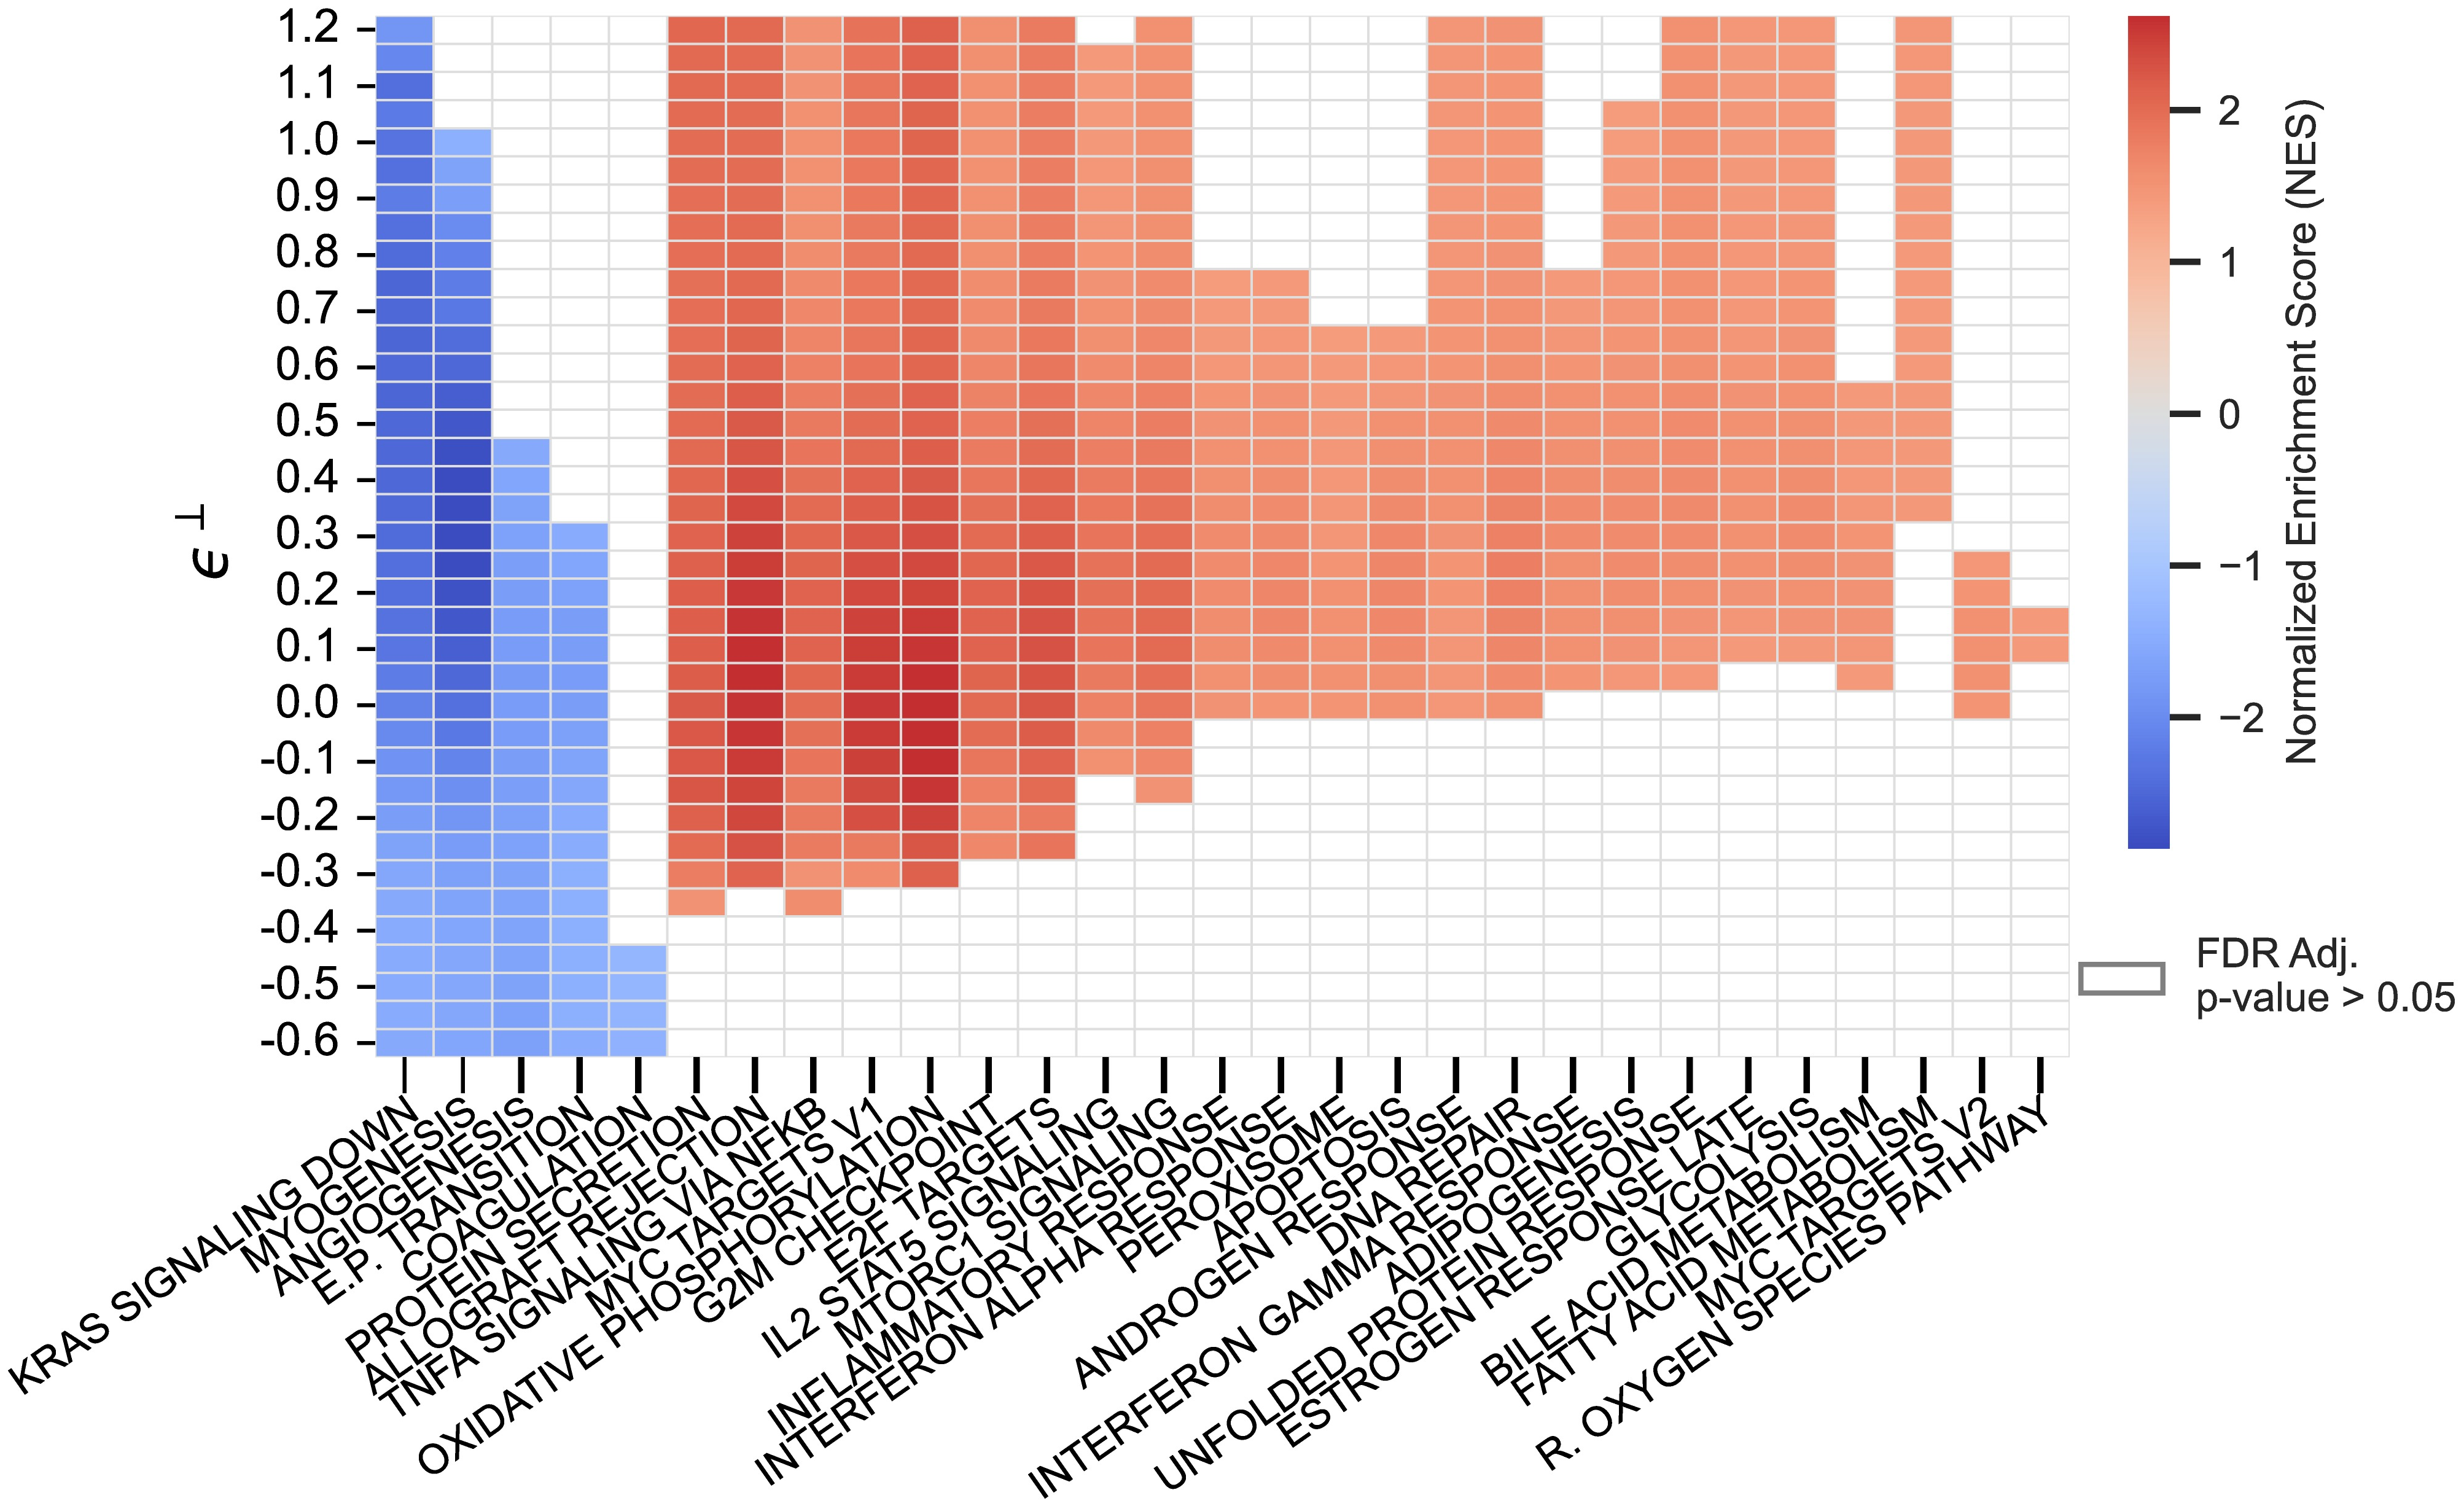
\includegraphics[width=0.9\linewidth]{./images/thyroid_lfc_sens.png}
\end{center}

\small \textcolor{gray}{McGovern, Nixon \& and Silverman (2023) Addressing Erroneous Scale Assumptions in Microbe and Gene Set Enrichment Analysis, \textit{PLoS Computational Biology}}
\note{
\begin{itemize}
\item how to read the plot
\end{itemize}

Make sure to really hit on ``does this matter''
\begin{itemize}
\item does this change any conclusions of aran et al?
\item If we were looking at this for first time, does this provide any new insight?
\begin{itemize}
\item Which sets to trust and which not too?
\item This plot lets reader decide.
\end{itemize}
\end{itemize}


Mention that we discovered that there are some gene sets that are significant for all values of \(\epsilon^{\perp}\). In our paper we use this to develop a hypothesis test that controls type-I error (and has non-zero power; power is not great but its remarkable its not zero given some of the theory michelle mentioned). See paper for explanation. Later we will highlight some ongoing work we are doing to boost the power.}
\end{frame}
\begin{frame}[label={sec:org6ffa9d4},fragile]{Software: Just 1 Exrtra Argument}

\begin{columns}
\begin{column}{0.5\columnwidth}
\begin{center}
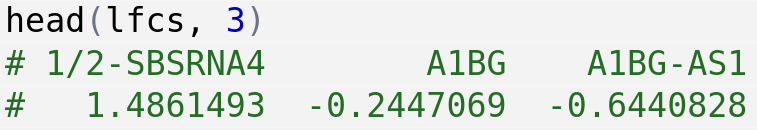
\includegraphics[width=0.85\linewidth]{./images/lfcs.png}
\end{center}
\end{column}
\begin{column}{0.5\columnwidth}
\begin{center}
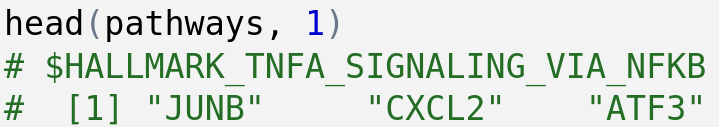
\includegraphics[width=0.85\linewidth]{./images/pathways.png}
\end{center}
\end{column}
\end{columns}

\begin{center}
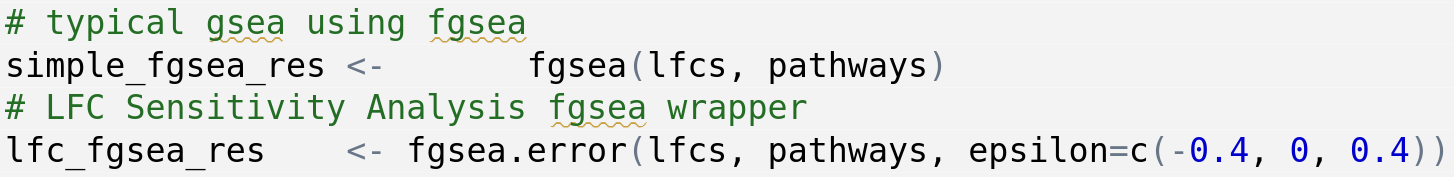
\includegraphics[width=1\linewidth]{./images/fgsea_example.png}
\end{center}

\pause
\begin{center}
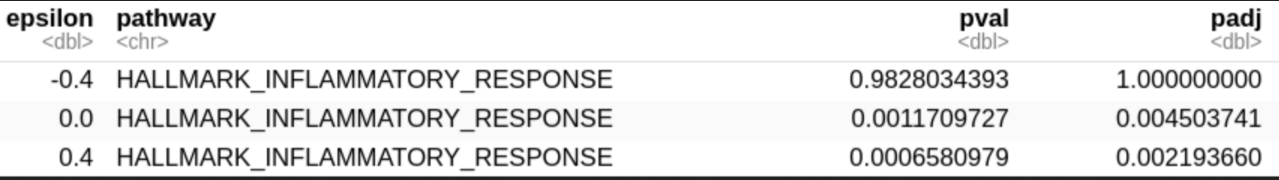
\includegraphics[width=1\linewidth]{./images/lfc_sens_output_small.png}
\end{center}


\note{Mention where software can be found. }
\end{frame}
\section{Inter-Entity Correlations}
\label{sec:orgdf10652}
\begin{frame}[label={sec:org813329d}]{Problem with Inter-Entity Correlations}
\begin{itemize}
\item Genes (and microbes) tend to be correlated.
\end{itemize}
\vfill
\begin{itemize}
\item Entity Label permutation test ignores these correlations.
\end{itemize}
\vfill
\begin{itemize}
\item This leads to elevated rates of false positives (Wu et al. 2012, \textit{Nucleic Acids Res})
\end{itemize}
\end{frame}
\begin{frame}[label={sec:orgb1ed9c2}]{GSEA with Sample Label Permutations (GSEA-S)}
\begin{itemize}
\item GSEA but we permute which samples are in case versus control.
\end{itemize}
\vfill
\begin{itemize}
\item Permutation based null models retains inter-entity correlations (addressing false positives)
\end{itemize}
\vfill
\pause
\begin{alertblock}{}
Can't run LFC Sensitivity Analysis for GSEA-S as described before because \(\hat{\theta}\) also changes when sample labels are permuted. 
\end{alertblock}
\vfill
\pause
\begin{block}{Updated LFC Sensitivity Analysis for GSEA-S}
Same as before but when sampling from null (permutation distribution) need to use
\[\phi_{S \text{ perm}}=u(\hat{\theta}_{\text{perm}} + \mathbf{1}\epsilon^{\perp})\]
\end{block}
\end{frame}
\begin{frame}[label={sec:org39578c9}]{Real Data Example}
  \begin{itemize}
  \item GSEA-S on NAT vs. Healthy Thyroid dataset revealed no positives (!)
    \pause
    \item Instead we performed an Updated LFC Sensitivity Analysis with GSEA-S using breast Tumor vs. Healthy tissue:
  \end{itemize}
  \begin{center}
    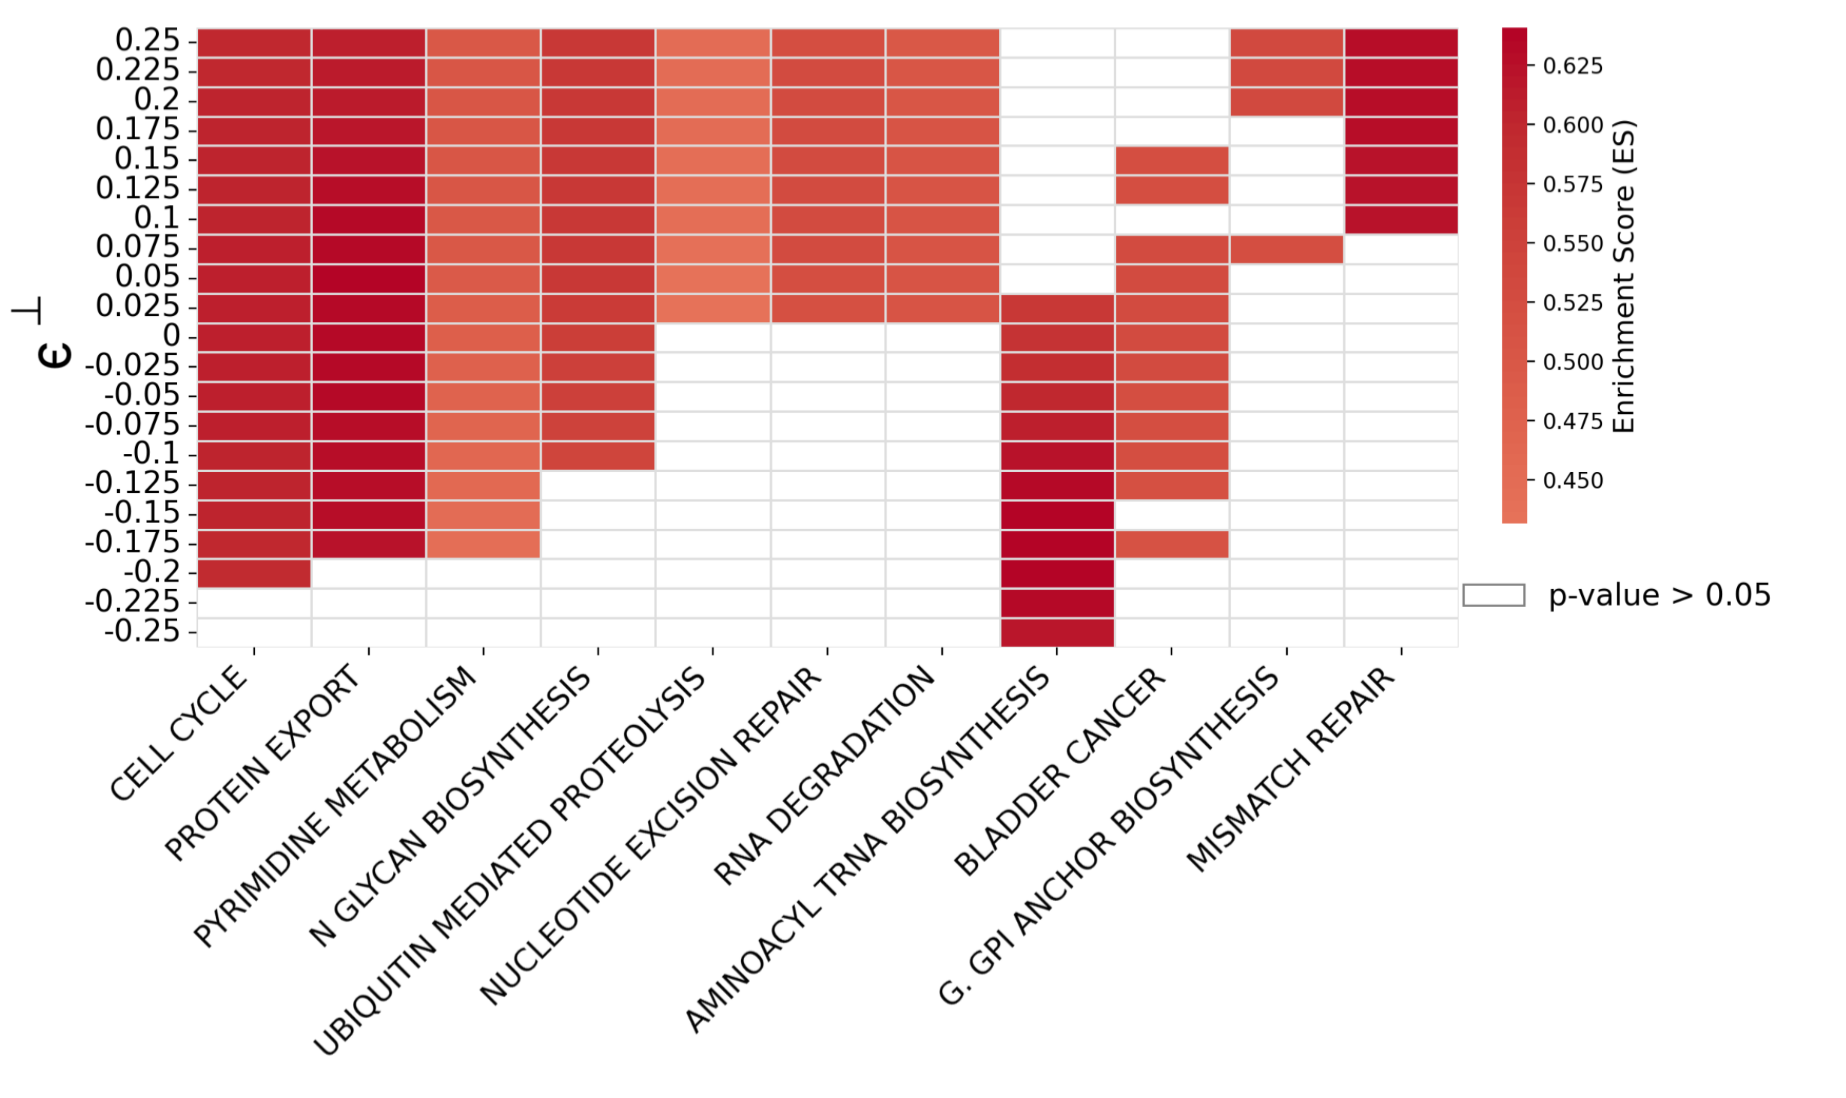
\includegraphics[width=0.85\linewidth]{./images/breast_data.png}
  \end{center}
\note{
In our paper we showed that the Aran et al. analysis, nothing is significant! Inter-gene correlations are important.

In our paper we also provided the above analysis on a different dataset to show that this type of sensitivity analysis still helps.}
\end{frame}
\begin{frame}[label={sec:or543}]{Software: Just 1 more argument}
   \begin{center}
    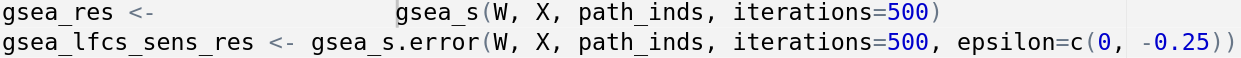
\includegraphics[width=1\linewidth]{./images/software_sl.png}
   \end{center}
   \begin{center}
    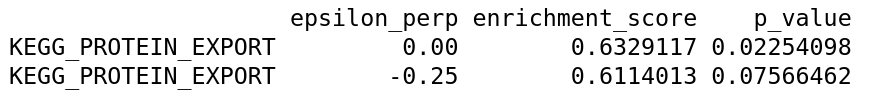
\includegraphics[width=1\linewidth]{./images/sl_output.png}
  \end{center} 
\end{frame}
\begin{frame}[label={sec:org224e0aa}]{Summary Recommendations}
\begin{description}
\item[{Few Samples (\(N<20\))}] Use GSEA (entity label permutations) and LFC Sensitivity Analysis
\end{description}
\vfill
\begin{description}
\item[{Many Samples (\(N\ge 20\))}] Use GSEA-S (sample label permutations) and Updated LFC Sensitivity Analysis
\end{description}
\end{frame}
\begin{frame}[label={sec:org8f90c24}]{Beyond GSEA and GSEA-S}
\begin{itemize}
\item Not all methods for DSA can be represented as \[\phi_{S}=u(\theta).\]
\end{itemize}
\vfill
\begin{itemize}
\item Some (e.g., CAMERA) can only be written as:  \[\phi_{S}=u(W)\]
\end{itemize}
\vfill
\begin{itemize}
\item See McGovern et al. (2023) \textit{PLoS Comp. Bio} for sensitivity analysis algorithm using scale models.
\end{itemize}
\note{
\begin{itemize}
\item There is no best method for DSA.
\item GSEA and GSEA-S are just two options.
\end{itemize}}
\end{frame}

\begin{frame}
  \frametitle{Acknowledgements}
  \begin{itemize}
    \item Dr. Justin Silverman (PI)
    \item Dr. Michelle Nixon
    \item Dr. Greg Gloor 
    \item Maxwell Konaris
    \item Tinghua Chen
    \item Won Gu
    \item Andrew Sugarman
    \item Manan Saxena
  \end{itemize}
\end{frame}

\section{Future Directions and Upcoming Works}
\label{sec:orgd3bb6eb}
\begin{frame}[label={sec:org3871889}]{Sparse Scale Simulation Random Variables}
\begin{itemize}
\item Scale Models discussed by Dr. Nixon involved quantifying uncertainty in \(\theta^{\perp}\) directly.
\end{itemize}
\vfill
\begin{itemize}
\item However if we know that only a few taxa are changing (a sparsity assumption), then more powerful scale models can be developed.
\end{itemize}
\vfill
\begin{itemize}
\item See Dr. Justin Silverman's talk Tuesday at 2:45pm in Clap Hall Auditorium for more information. \textit{Sparse Approaches to Differential Abundance and Expression Analyses: Potential and Pitfalls}
\end{itemize}
\end{frame}
\begin{frame}[label={sec:orgbca61bb}]{Covariance / Network Inference}
\begin{itemize}
\item We have focused on LFC and DSA estimands.
\end{itemize}
\vfill
\begin{itemize}
\item Many research want to estimate networks and interactions between genes or taxa.
\end{itemize}
\vfill
\begin{itemize}
\item Core to these methods is covariance estimation
\end{itemize}
\[\Sigma_{d_{1}, d_{2}}=\text{Cov}(\log W_{d_{1} \cdot}, \log W_{d_{2} \cdot}).\]
\vfill
\begin{itemize}
\item Current methods (including proportionality) suffer from substantial unacknowledged bias.
\end{itemize}
\vfill
\begin{itemize}
\item We are developing Bayesian and Frequentist methods that address this problem.
\end{itemize}
\end{frame}
\begin{frame}[label={sec:org4ec3de6}]{Powerful Frequentist Hypothesis Tests for DA/DE}
  \begin{itemize}
  \item Bayesian scale models as discussed by Dr. Nixon require defining a distribution of uncertainty over the scale:
    \begin{align*}
      \theta^\perp \sim \mathcal{N}(0, \sigma^2).
    \end{align*}

\item We are developing a Frequentist framework where scale uncertainty is incorporated as bounds:
  \begin{align*}
    \theta ^\perp \in [\theta^\perp_l, \theta^\perp_u].
  \end{align*}

\item This framework allows for the development of novel, Frequentist hypothesis tests in differential expression and differential abundance:
  \begin{align*}
    H_0: \theta_d = 0.
  \end{align*}
 \end{itemize} 
\end{frame}
\end{document}
